% !TEX root = ../VPJ.tex

\chapter{Visualisierung}
\label{sec:Visualisierung}

\section{Grundstruktur}

Coorporate Design

\begin{figure}[htb]
    \centering
    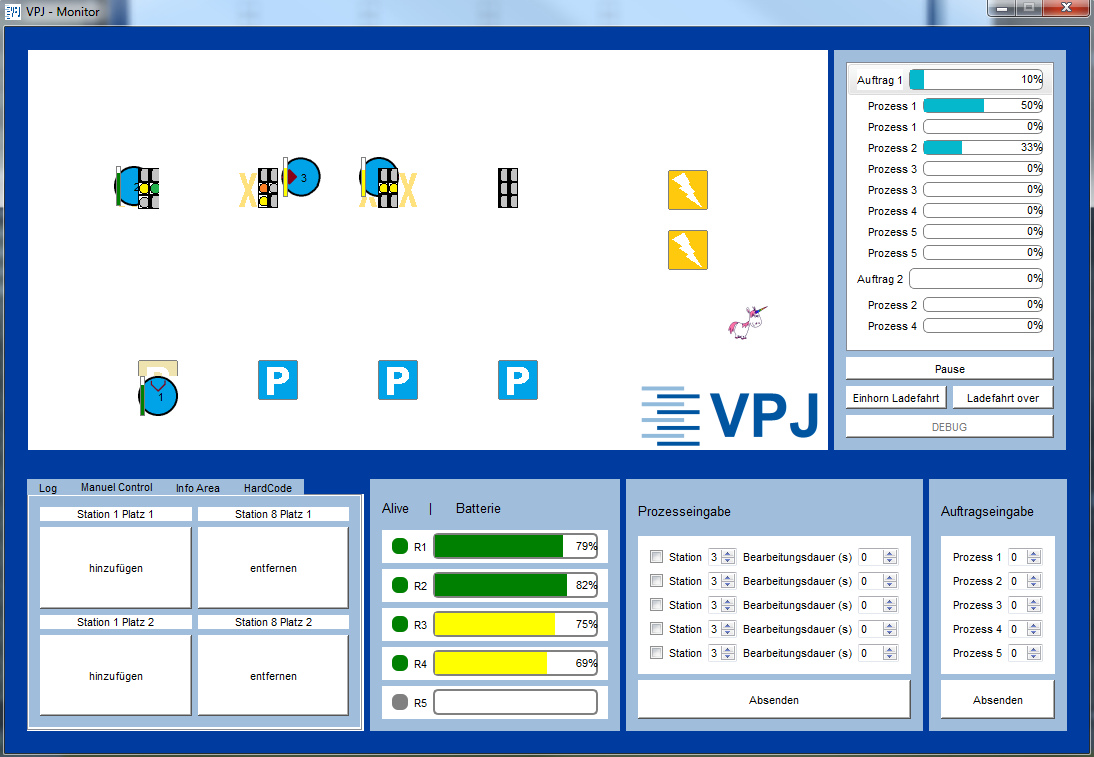
\includegraphics[width=1\textwidth]{Abbildungen/Gesamtprogramm.png}
    \caption{Übersicht Visualisierung}		
    \label{fig:Gesamtprogramm}
\end{figure}

\begin{figure}[htb]
    \centering
    \includegraphics[width=1\textwidth]{Abbildungen/GesamtprogrammROT.png}
    \caption{Übersicht Visualisierung im Hard-Code Modus}		
    \label{fig:GesamtprogrammROT}
\end{figure}

\section{Live-View}

\begin{figure}[htb]
    \centering
    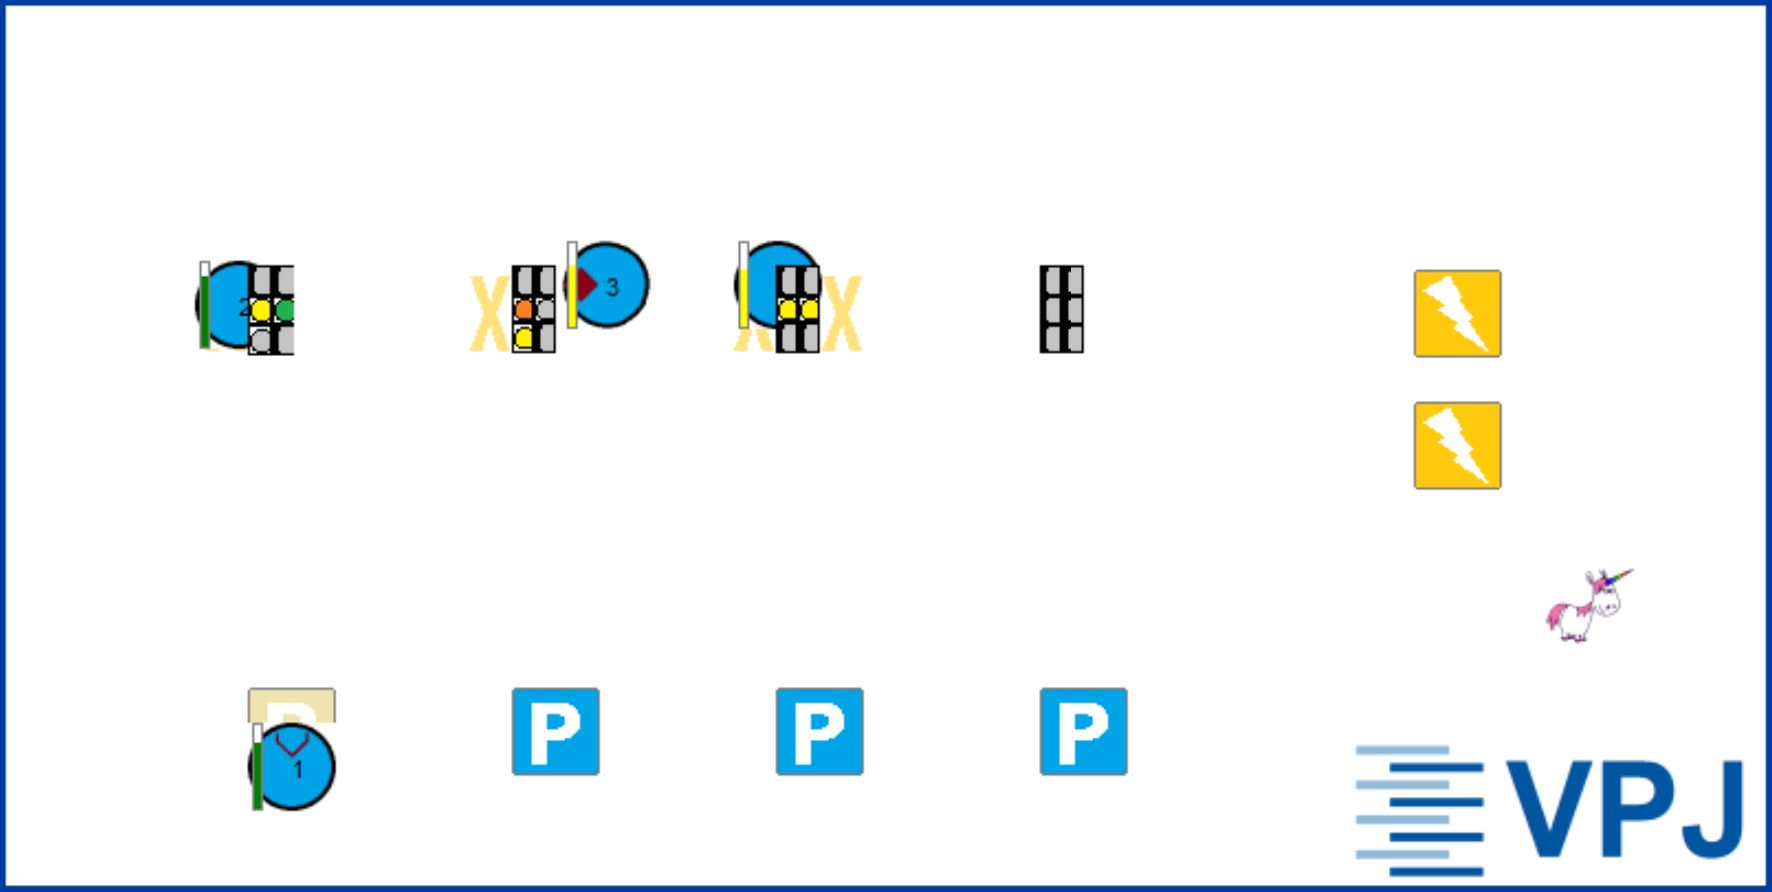
\includegraphics[width=0.9\textwidth]{Abbildungen/LiveView.png}
    \caption{Visualisierung Live-View}		
    \label{fig:LiveView}
\end{figure}

\begin{figure}[htb]
    \centering
    
\includegraphics[width=0.4\textwidth]{Abbildungen/Parkplatz.png}
    \caption{Visualisierung Parkplatz}		
    \label{fig:Parkplatz}
\end{figure}

\begin{figure}[htb]
    \centering
    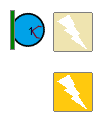
\includegraphics[width=0.25\textwidth]{Abbildungen/Laden.png}
    \caption{Visualisierung Ladestation}		
    \label{fig:Ladestation}
\end{figure}

\begin{figure}[htb]
    \centering
    
\includegraphics[width=0.2\textwidth]{Abbildungen/Station.png}
    \caption{Station mit verschiedenen Arbeitsplatzstati}		
    \label{fig:Station}
\end{figure}

\begin{figure}[htb]
    \centering
    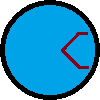
\includegraphics[width=0.1\textwidth]{Abbildungen/RobotinoGoffen.png}
    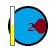
\includegraphics[width=0.1\textwidth]{Abbildungen/RobotinoGZu.png}
    
\includegraphics[width=0.1\textwidth]{Abbildungen/RobotinoDefect.png}
    \caption{Roboter in verschiedenen Stati (vlnr: Greifer offen, Greifer geschlossen, Defekt)}		
    \label{fig:Robotino}
\end{figure}

\section{Auftragsübersicht}
\label{sec:Auftragsuebersicht}

\begin{figure}[htb]
    \centering
    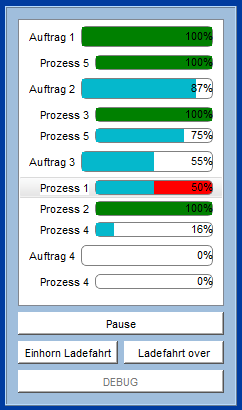
\includegraphics[width=0.4\textwidth]{Abbildungen/Auftragsfortschritt.png}
    \caption{Auftragsfortschritt}		
    \label{fig:Auftragsfortschritt}
\end{figure}

\begin{figure}[htb]
    \centering
    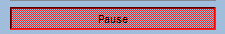
\includegraphics[width=0.4\textwidth]{Abbildungen/Pause.png}
    \caption{Pause Button gedrückt}		
    \label{fig:Pause}
\end{figure}

\section{Tab-View}

\begin{figure}[htb]
    \centering
    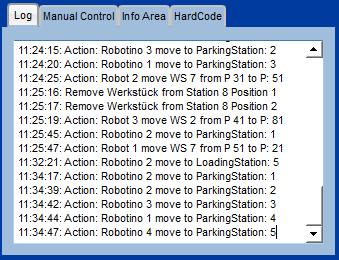
\includegraphics[width=0.6\textwidth]{Abbildungen/Log.png}
    \caption{Tab: Log View}		
    \label{fig:Log}
\end{figure}

\begin{figure}[htb]
    \centering
    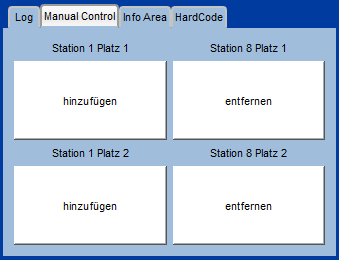
\includegraphics[width=0.6\textwidth]{Abbildungen/ManualControl.png}
    \caption{Tab: Manual Control}		
    \label{fig:ManualControl}
\end{figure}

\begin{figure}[htb]
    \centering
    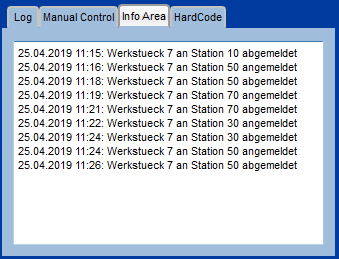
\includegraphics[width=0.4\textwidth]{Abbildungen/TimestampsWerkstueck.png}
    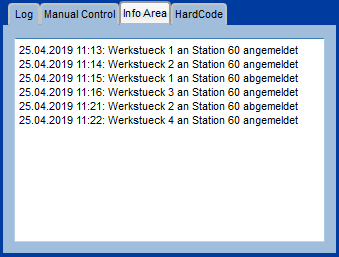
\includegraphics[width=0.4\textwidth]{Abbildungen/TimestampsStation.png}
    \caption{Tab: Info Area}		
    \label{fig:InfoArea}
\end{figure}

\subsection{Hard-Code Bereich}
\label{sec:HardCode}

\begin{figure}[htb]
    \centering
    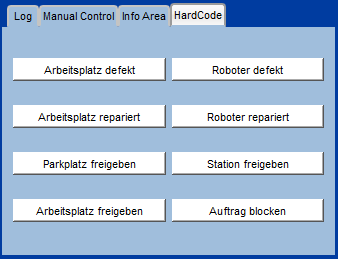
\includegraphics[width=0.6\textwidth]{Abbildungen/HardCode.png}
    \caption{Tab: Hard-Code}		
    \label{fig:HardCode}
\end{figure}

\section{Roboterstatus}

\begin{figure}[htb]
    \centering
    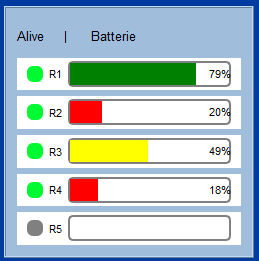
\includegraphics[width=0.5\textwidth]{Abbildungen/Batterie.png}
    \caption{Batterie und Statusanzeige}		
    \label{fig:Batterie}
\end{figure}

\begin{figure}[htb]
    \centering
    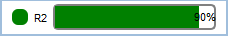
\includegraphics[width=0.4\textwidth]{Abbildungen/BatterieAlive1.png}
    
\includegraphics[width=0.4\textwidth]{Abbildungen/BatterieAlive2.png}
    \caption{Roboterstatus-LED blinkend}		
    \label{fig:Led}
\end{figure}

\section{Prozesseingabe}
\label{sec:Prozesseingabe}

\begin{figure}[htb]
    \centering
    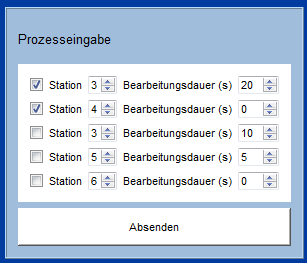
\includegraphics[width=0.5\textwidth]{Abbildungen/Prozesseingabe.png}
    \caption{Visualisierung - Prozesseingabe}		
    \label{fig:Prozesseingabe}
\end{figure}

\section{Auftragseingabe}
\label{sec:Auftragseingabe}

\begin{figure}[htb]
    \centering
    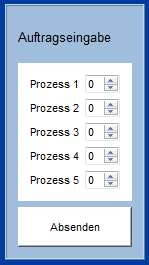
\includegraphics[width=0.25\textwidth]{Abbildungen/Auftragsvergabe.png}
    \caption{Visualisierung - Auftragsvergabe}		
    \label{fig:Auftragsvergabe}
\end{figure}


\section{Benutzerinteraktion}

\subsection{Tooltips}
\label{sec:tooltips}
\inlinetodo {Tooltips mit Bildern her und erlaeeeren}


